\documentclass{beamer}
\usepackage[italian]{babel} % lingua 
\usepackage[latin1]{inputenc} % codifica
\usepackage{amsmath} % equazioni 
\usepackage{amsthm} % teoremi
\usepackage{amssymb} % simboli matematici
\usepackage{graphicx, subfigure}
\usepackage[T1]{fontenc}
\usepackage{bookmark}
\usepackage{graphicx}
\usepackage{physics}
\usepackage{animate}
\usepackage{graphicx}
\usepackage{changepage}  
\newlength{\offsetpage}
\setlength{\offsetpage}{1.0cm}
\newenvironment{widepage}{\begin{adjustwidth}{-\offsetpage}{-\offsetpage}%
    \addtolength{\textwidth}{2\offsetpage}}%
{\end{adjustwidth}}

\usepackage{tikz}
\usepackage{color}
\usepackage{epstopdf}
\usepackage{multirow}
\usenavigationsymbolstemplate{}
\usetikzlibrary{positioning}
\usetikzlibrary{trees,arrows}

\newcommand{\bea}{\setlength{\jot}{10pt}\begin{eqnarray*}}
\newcommand{\eea}{\end{eqnarray*}}
\usepackage{tensind}
\tensordelimiter{:}


\usefonttheme{professionalfonts}

\title{Analyzing Gravitational Waves \\ through Numerical Simulations}
\author{Lorenzo Speri}
%\date{17$^{th}$ July 2017}
\institute[]{Department of Physics \\
University of Trento\\
17th July 2018}

\usetheme{Singapore}
\setbeamercovered{dynamic}
\theoremstyle{definition}
\newtheorem{definizione}{Definition}
\theoremstyle{plain}
\newtheorem{proposition}{Proposition}
\logo{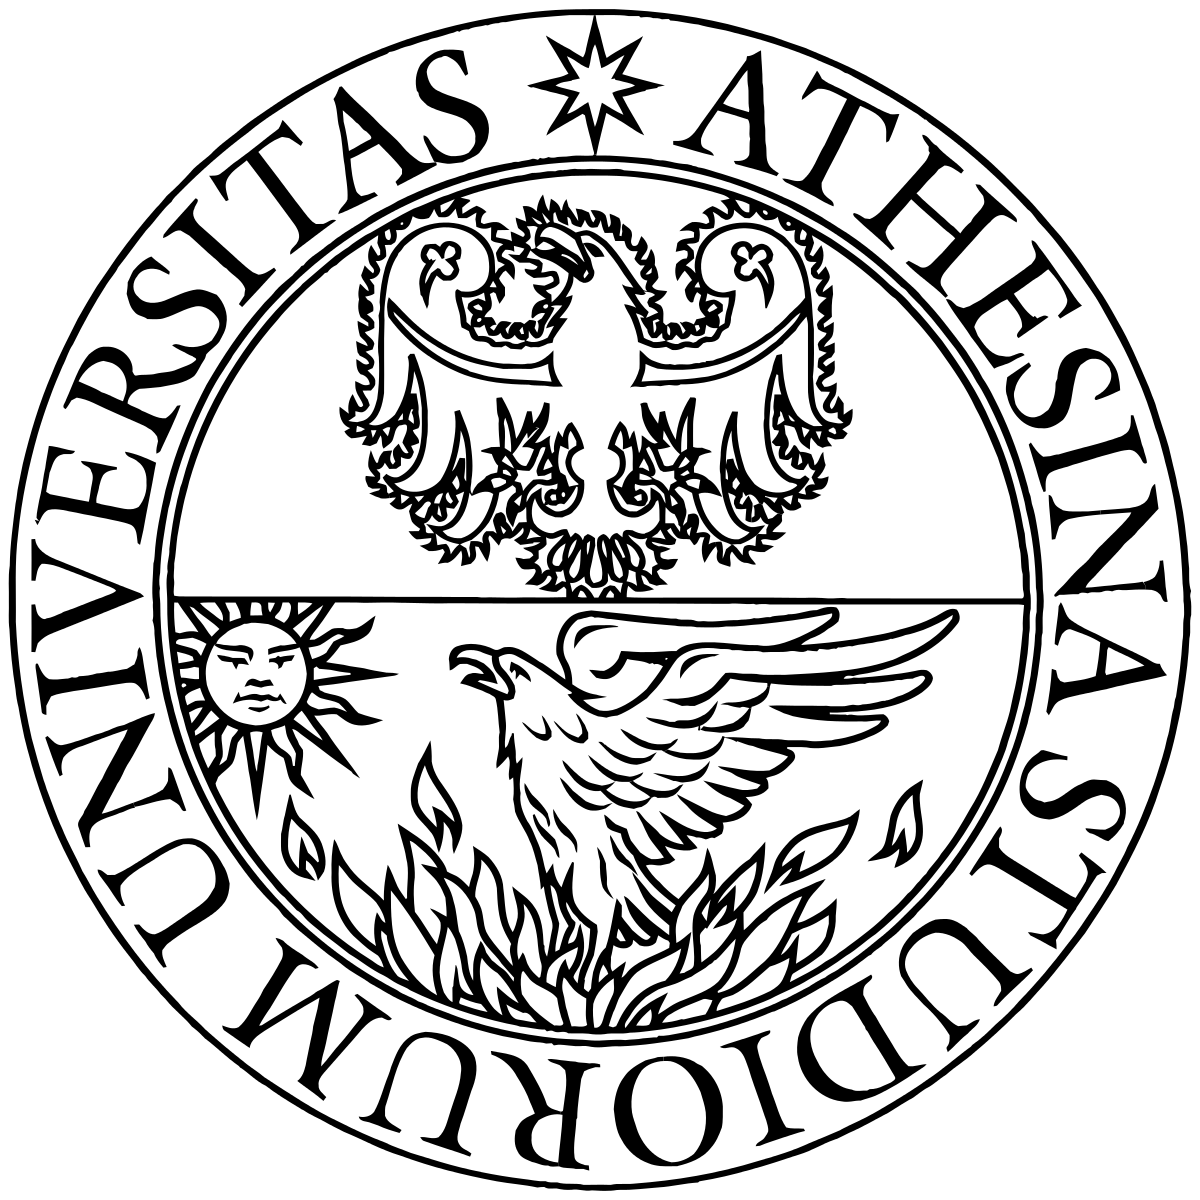
\includegraphics[width=0.09\textwidth]{logo.png}}
\setbeamertemplate{footline}[frame number]
\begin{document}
\tikzstyle{level 1}=[level distance=5.5cm, sibling distance=5.5cm]
\tikzstyle{level 2}=[level distance=4.5cm, sibling distance=1.5cm]
\tikzstyle{bag} = [text width=4em, text centered]
\tikzstyle{end} = [rectangle, draw=#1, minimum width=3pt, inner sep=6pt]
\begin{frame}
	\begin{figure}
		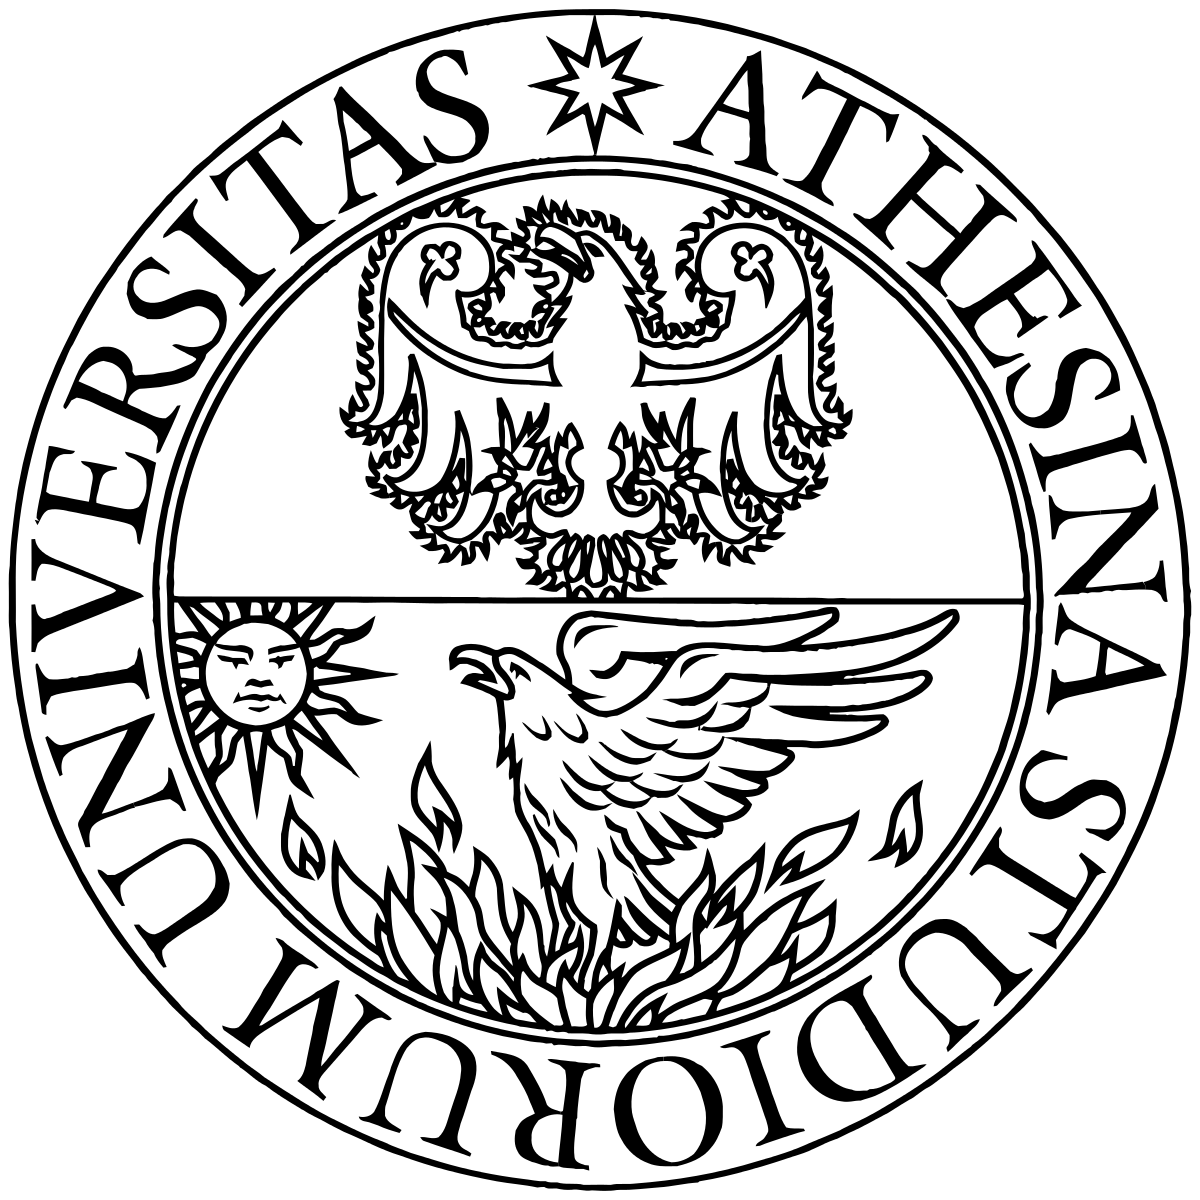
\includegraphics[width=0.30\textwidth]{logo.png}
	\end{figure}
	\maketitle	
\end{frame}
\begin{frame}{Contents}
	\begin{enumerate}
		\item Introduction \\
		\vspace{0.2cm}
		\item Einstein's Field Equation \\
		\vspace{0.2cm}
		\item Effects of Gravitational Waves \\
		\vspace{0.2cm}
		\item Production of Gravitational Waves \\
		\vspace{0.2cm}
		\item Numerical Evolution of Compact Binaries
		\vspace{0.2cm}
		\item Conclusions
	\end{enumerate}
\end{frame}

\section{Introduction}
\begin{frame}{Why Gravitational Waves?}
The speed of light is the speed of causality.\\
\vspace{0.7cm}
Gravity must be causal.\\
\vspace{0.7cm}
A change in a gravitating source is communicated to a distant observer not faster than light.\\
\vspace{0.7cm}
Communication of a change in spacetime $\rightarrow$ Gravitational Waves
\end{frame}

\section{Einstein's Field Equation}
\subsection{}
\begin{frame}{Einstein's Field Equation}
	Einstein's Field Equation is a rather complicated tensor equation
	\vspace{0.8cm}
	\\
	\[
	R_{\mu \nu} - \dfrac{1}{2} R g_{\mu \nu} = 
\dfrac{8 \pi G}{c^4} T_{\mu \nu}
	\]
	\vspace{0.8cm}
	\\
	where
\bea
\Gamma ^{\alpha} _{\beta \gamma} = 
\dfrac{1}{2} g^{\alpha \rho} \qty(
\partial_\beta g_{\gamma \rho} + 
\partial_\gamma g_{\rho \beta} -
\partial_\rho g_{\beta \gamma}
)
\\
: R^\alpha _{\beta \gamma \sigma}:
=
:\Gamma ^\alpha _{\gamma \lambda}:\,
:\Gamma ^\lambda _{\sigma \beta}:
-
:\Gamma ^\alpha _{\sigma \lambda}:\,
:\Gamma ^\lambda _{\gamma \beta}:
+
\partial_\gamma :\Gamma^\alpha _{\sigma \beta}: 
-
\partial_\sigma :\Gamma^\alpha _{\gamma \beta} :
\\
R_{\mu \nu} = :R^\alpha _\mu \alpha _\nu: \hspace{1.5cm}
R=\eta^{\mu \nu} R_{\mu \nu} = :R^{\mu} _\mu:
\eea	
\end{frame}

\begin{frame}{Linearized Einstein's Field Equation}
\begin{itemize}
\item Weak field linearized approximation
	\[
	g_{\mu \nu} = \eta_{\mu \nu} + h_{\mu \nu} \hspace{1.5cm}
	\abs{h_{\mu \nu}}\ll 1
	\]
\item Trace-reversed perturbation metric
\[
\bar{h} _{\mu \nu} = h_{\mu \nu} - \dfrac{1}{2} h \eta_{\mu \nu} \hspace{1.5cm} \bar{h}=\bar{h}^{\mu \nu} \eta_{\mu \nu} = - h
\]
\item Lorenz gauge $\partial_{\mu} h^{\mu \nu}=0$\\ 
\end{itemize}
leads to the linearized Einstein's field equation
\\
\vspace{0.3cm}
\[
\qty(
\dfrac{1}{c^{2}}
\pdv[2]{}{t}
-
\nabla ^{2}
)
\bar{h} _{\mu \nu} =\dfrac{16 \pi G}{c^{4}} T_{\mu \nu}
\]
\end{frame}

\begin{frame}{Linearized Einstein's Field Equation $T_{\mu \nu} =0$}
In vacuum $T_{\mu \nu}=0$
\[
\qty(
\dfrac{1}{c^{2}}
\pdv[2]{}{t}
-
\nabla ^{2}
)
\bar{h} _{\mu \nu} =0
\]
\vspace{1cm}
Plane wave solution 
\[
\bar{h}_{\mu \nu} = A_{\mu \nu} \cos\qty[i\omega ( t- z/c)]
\]
\end{frame}

\begin{frame}{Radiative degrees of freedom}
The conditions imposed by the Transverse Traceless gauge
\[
h^{\text{TT}}_{0 \nu} = 0 \qquad
\eta ^{\mu \nu } h^{\text{TT}}_{\mu \nu} =0
\qquad
\partial^{\mu} h^{\text{TT}} _{\mu \nu}=0
\]
allow us to obtain the only two radiative degrees of freedom
\[
\bar{h}^{\text{TT}}_{\mu \nu} =
\begin{bmatrix}
0 & 0 & 0 & 0 \\
0 & h_{+} & h_{\times} & 0 \\
0 & h_{\times} & -h_{+} & 0 \\
0 & 0 & 0 & 0 \\
\end{bmatrix}
\]
where 
\bea
h_{+} = A _{11} \cos \qty(\omega(t-z/c)) \\
h_{\times} =  A _{12} \cos \qty(\omega(t-z/c))
\eea
\end{frame}


\section{Effects of GWs}
\subsection{}
\begin{frame}{Geodesic Deviation Equation}
For slowly-moving free-falling particles the geodesic deviation equations become
\bea
\pdv[2]{}{t} S^{1} &=& \dfrac{1}{2} S^{1} \pdv[2]{}{t} h_{+} + \dfrac{1}{2} S^{2} \pdv[2]{}{t} h_{\times} \\
\pdv[2]{}{t} S^{2} &=& \dfrac{1}{2} S^{1} \pdv[2]{}{t} h_{\times} - \dfrac{1}{2} S^{2} \pdv[2]{}{t} h_{+}
\eea
first order solution
\bea
S^{1} = S^{1}(t=0) \qty(1 + \dfrac{1}{2} h_{+})+ \dfrac{1}{2} h_{\times} S^{2}(t=0) \\
S^{2} = S^{2}(t=0) \qty(1 - \dfrac{1}{2} h_{+}) +  \dfrac{1}{2} h_{\times} S^{1}(t=0)
\eea
\end{frame}




\begin{frame}{$+$ polarization $h_{\times}=0$}
	\begin{figure}
    \centering
    \animategraphics[loop,autoplay,scale=0.5]{12}{/Users/lorenzosperi/Documents/GitHub/thesis/gw/plus_pol/frame-}{0}{62}
    \end{figure}
\end{frame}

\begin{frame}{$\times$ polarization $h_{+}=0$}
	\begin{figure}
    \centering
    \animategraphics[loop,autoplay,scale=0.5]{12}{/Users/lorenzosperi/Documents/GitHub/thesis/gw/times_pol/frame-}{0}{62}
    \end{figure}
\end{frame}

\begin{frame}{Left-handed polarization}
	\begin{figure}
    \centering
    \animategraphics[loop,autoplay,scale=0.5]{12}{/Users/lorenzosperi/Documents/GitHub/thesis/gw/l_pol/frame-}{0}{62}
    \end{figure}
\end{frame}

\begin{frame}{Right-handed polarization}
	\begin{figure}
    \centering
    \animategraphics[loop,autoplay,scale=0.5]{12}{/Users/lorenzosperi/Documents/GitHub/thesis/gw/r_pol/frame-}{0}{62}
    \end{figure}
\end{frame}

\section{Production of GWs}
\subsection{}
\begin{frame}{Linearized Einstein's Field Equation $T_{\mu \nu} \neq  0$}
\[
\qty(
\dfrac{1}{c^{2}}
\pdv[2]{}{t}
-
\nabla ^{2}
)
\bar{h} _{\mu \nu} =\dfrac{16 \pi G}{c^{4}} T_{\mu \nu}
\]
\vspace{1cm}

\begin{itemize}
\item \textbf{far field approximation}%: the metric perturbation $\bar{h}_{\mu \nu}$ is evaluated at large distances $r$ from the source.
\vspace{0.3cm}
\item \textbf{slowly moving source}%: the light traverses the source much faster than the components of the source itself do.
\vspace{0.3cm}

\item \textbf{isolated system}%: the source of the gravitational radiation is an isolated and compact.

\end{itemize}
\end{frame}

\begin{frame}{Quadrupole Formula}
A solution of the Linearized Einstein's Field equation is the Quadrupole Formula
\bea
h^{\text{TT}}_{ij} = \dfrac{2G}{c^{4}r} \dv[2]{\mathcal{I}_{kl}(t_r)}{t} \qty(:P_{i}^{k}::P_{j}^{l}: - \dfrac{1}{2} P_{ij} P^{kl})
\eea
where
\[
\mathcal{I} _{kj} = \int \rho(\vb{y}) \qty(y_{k} y_{j} - \dfrac{1}{3}\delta_{kj} y^{l} y_{l} ) \; \dd[3] y
\]
and
\[
P_{i j} = \delta_{i j} - n_{i} n_{j}
\]
\end{frame}

\begin{frame}{slowly-moving equal-mass binary system}
For an equal-mass binary system rotating at angular frequency $\omega$ and orbital radius $R$, the quadrupole formula becomes
\[
h^{\text{TT}} _{ij} = \frac{8\,G M \,R^{2} \omega^{2}}{c^{4}\, r} \,
\begin{bmatrix}
- \cos 2 \omega t_r   &
 - \sin 2 \omega t_r &
0
\\
  -\sin 2 \omega t_r &
 \cos 2 \omega t_r &
0
\\
0 & 0 & 0\\
\end{bmatrix}
\]
estimate of the amplitude
\[
\frac{8\,G M \,R^{2} \omega^{2}}{c^{4}\, r} = 1.6 \times 10^{-22}
\]
setting $M=M_{\odot}=2 \times 10^{30}$ kg, $\omega=\sqrt{GM/(4R^{3})}$, $R = 3r_s=8.86 $ km and $r =100$ Mpc.
\end{frame}

\begin{frame}{slowly-moving equal-mass binary system}
\begin{figure}
    \centering
    \animategraphics[loop,autoplay,scale=0.5]{12}{/Users/lorenzosperi/Documents/GitHub/thesis/gw/gw_travelling/frame-}{0}{41}
    \end{figure}
\end{frame}


\section{Numerical Evolution}
\subsection{}
\begin{frame}{Numerical Evolution of Compact Binaries}
Quasi-equilibrium initial conditions of compact objects
\vspace{1cm}
\begin{itemize}
\item \textbf{Binary Black Holes (BBH)}
%\begin{table}
%\centering
%\begin{tabular}{|c|c|c|c|}
%\hline 
%simulation name & \texttt{par\_b} & \texttt{par\_m\_plus} & \texttt{par\_P\_plus[1]} \\ 
%\hline 
%BBH-b3 & 3 & 0.47656
% & +0.13808 \\ 
%%\hline 
%BBH-b4 & 4 & 0.48243 & +0.11148 \\ 
%%\hline 
%BBH-b5 & 5 & 0.48595 & +0.095433 \\ 
%%\hline 
%BBH-b6 & 6 & 0.48830 & +0.084541 \\ 
%%\hline 
%BBH-b7 & 7 &  0.48997 & +0.076578 \\ 
%%\hline 
%BBH-b10 & 10 & 0.49299 & +0.061542 \\ 
%\hline 
%\end{tabular} 
%\end{table}
\vspace{0.5cm}
\item \textbf{Binary Neutron Stars (BNS)}
	\end{itemize}
	\vspace{1cm}

\textbf{Gravitational Radiation}
$\Leftrightarrow$
\textbf{Dynamical Evolution}
\end{frame}

\begin{frame}{BBH-b3}
\begin{figure}
    \centering
    \animategraphics[loop,autoplay,scale=0.5]{8}{/Users/lorenzosperi/Documents/GitHub/thesis/gw/bbh-b3/frame-}{1}{216}
    \end{figure}
\end{frame}

\begin{frame}{BBH-b4}
\begin{figure}
    \centering
    \animategraphics[loop,autoplay,scale=0.5]{16}{/Users/lorenzosperi/Documents/GitHub/thesis/gw/bbh-b4/frame-}{1}{339}
    \end{figure}
\end{frame}

\begin{frame}{BBH-b5}
\begin{figure}
    \centering
    \animategraphics[loop,autoplay,scale=0.5]{24}{/Users/lorenzosperi/Documents/GitHub/thesis/gw/bbh-b5/frame-}{1}{739}
    \end{figure}
\end{frame}

\begin{frame}{BBH-b6, BBH-b7, BBH-b10}
\begin{widepage}
\begin{figure}
    \centering
    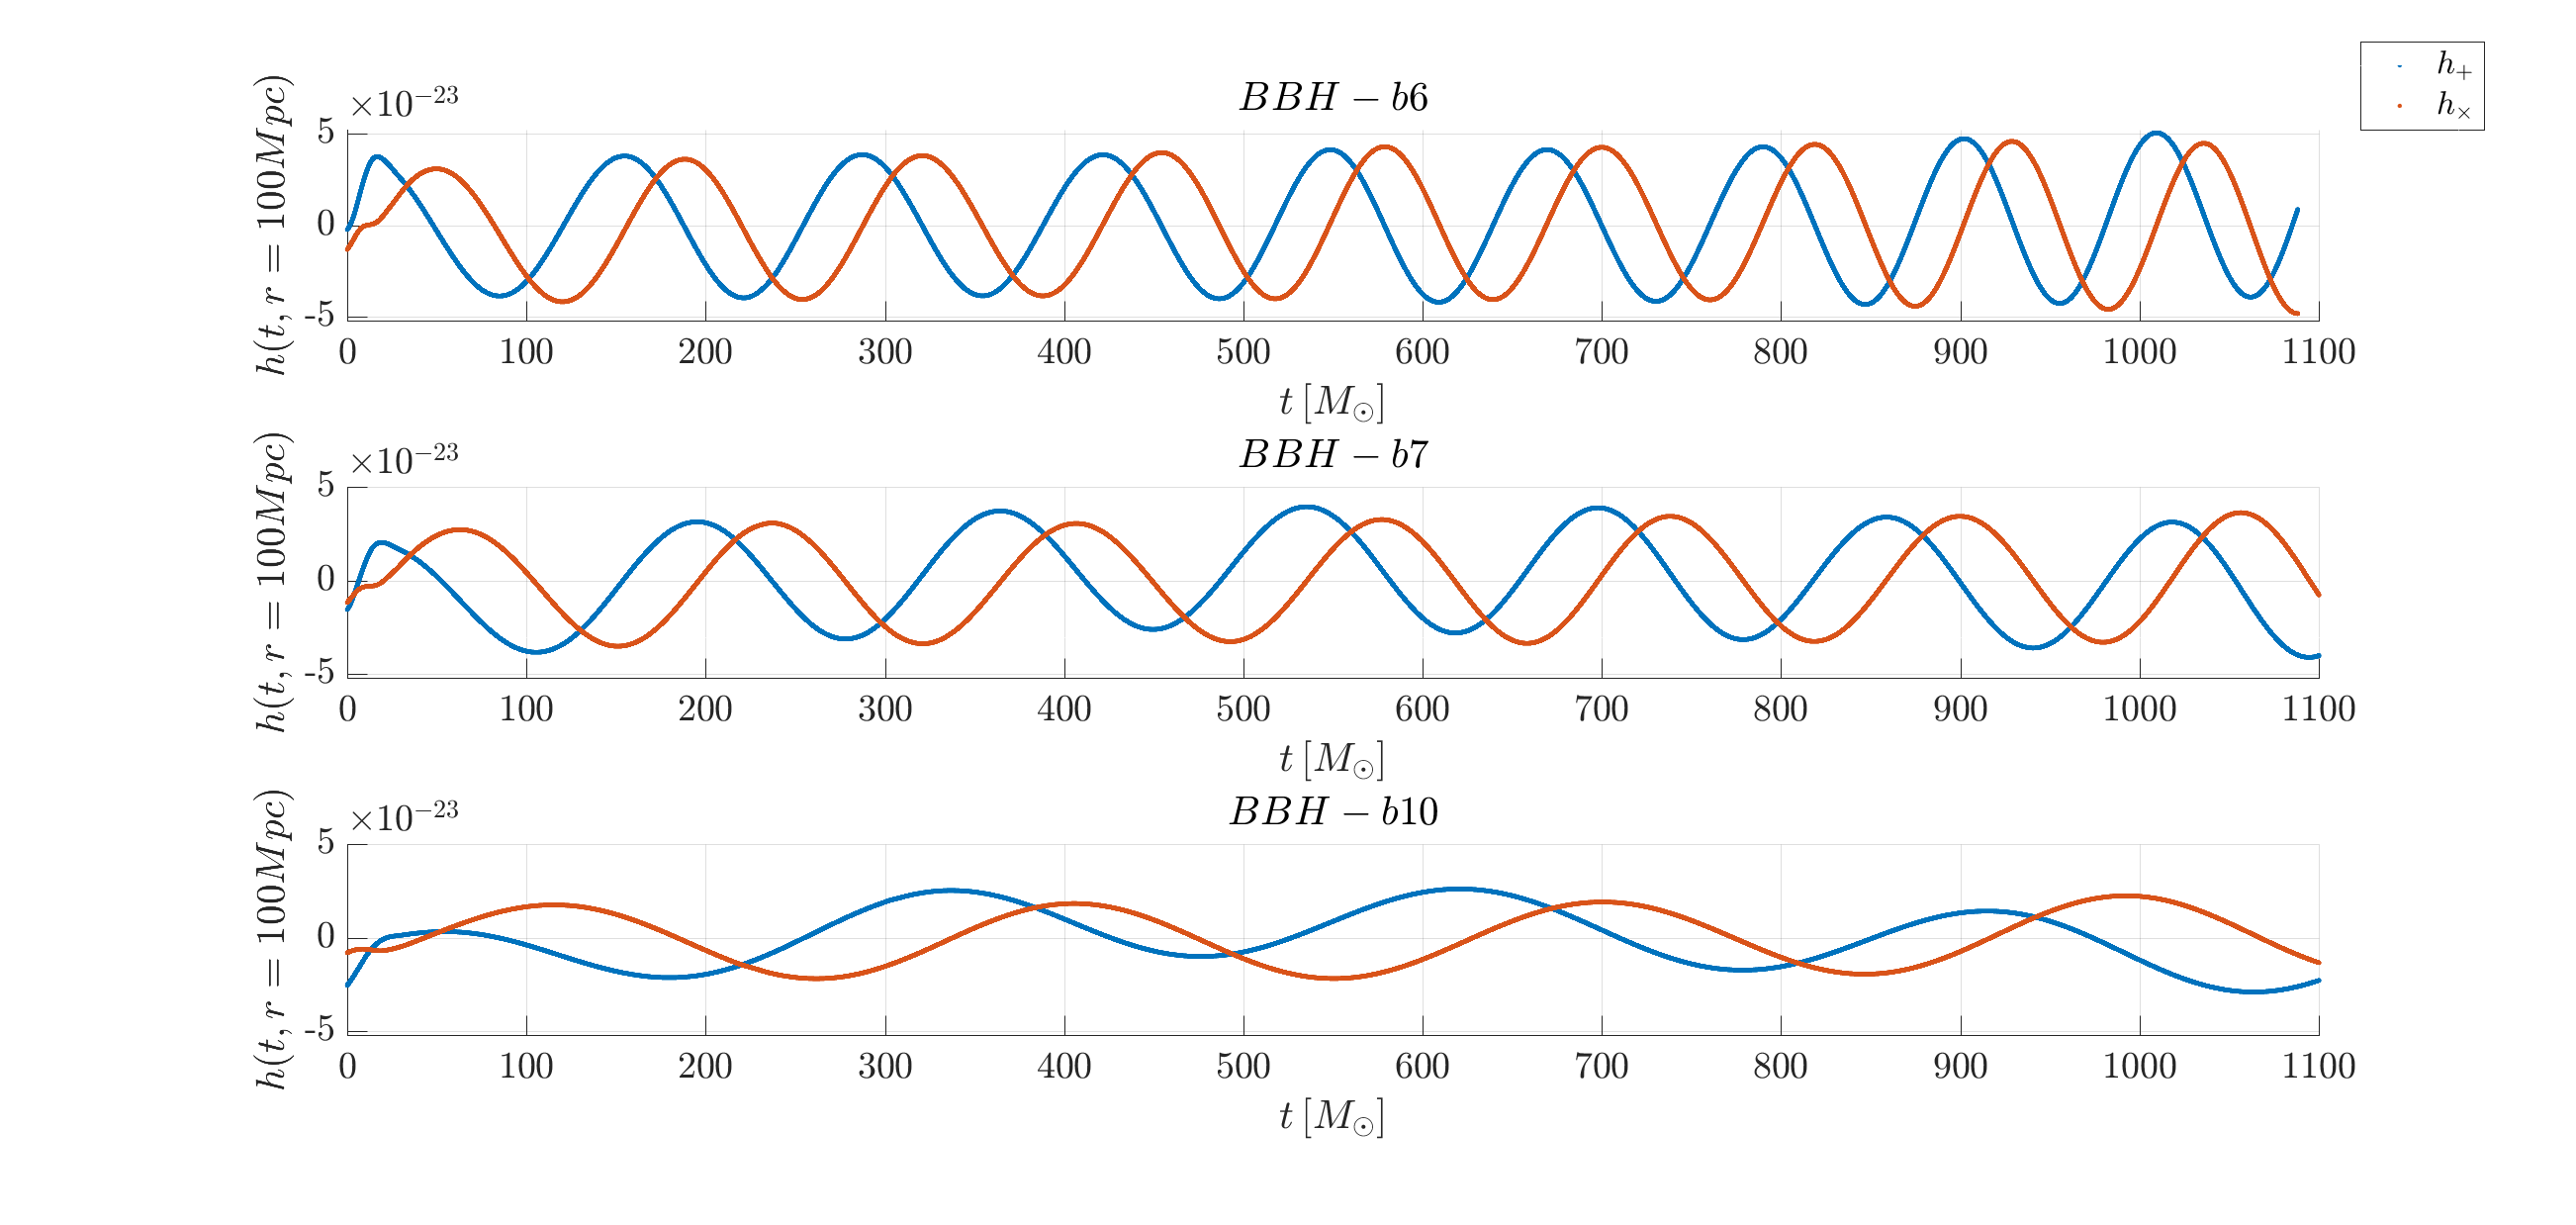
\includegraphics[scale=0.3,width=0.97\textwidth]{bbh-b6710.eps}
    \end{figure}
    \end{widepage}
\end{frame}

\begin{frame}{BNS}
\begin{widepage}
\begin{figure}
    \centering
    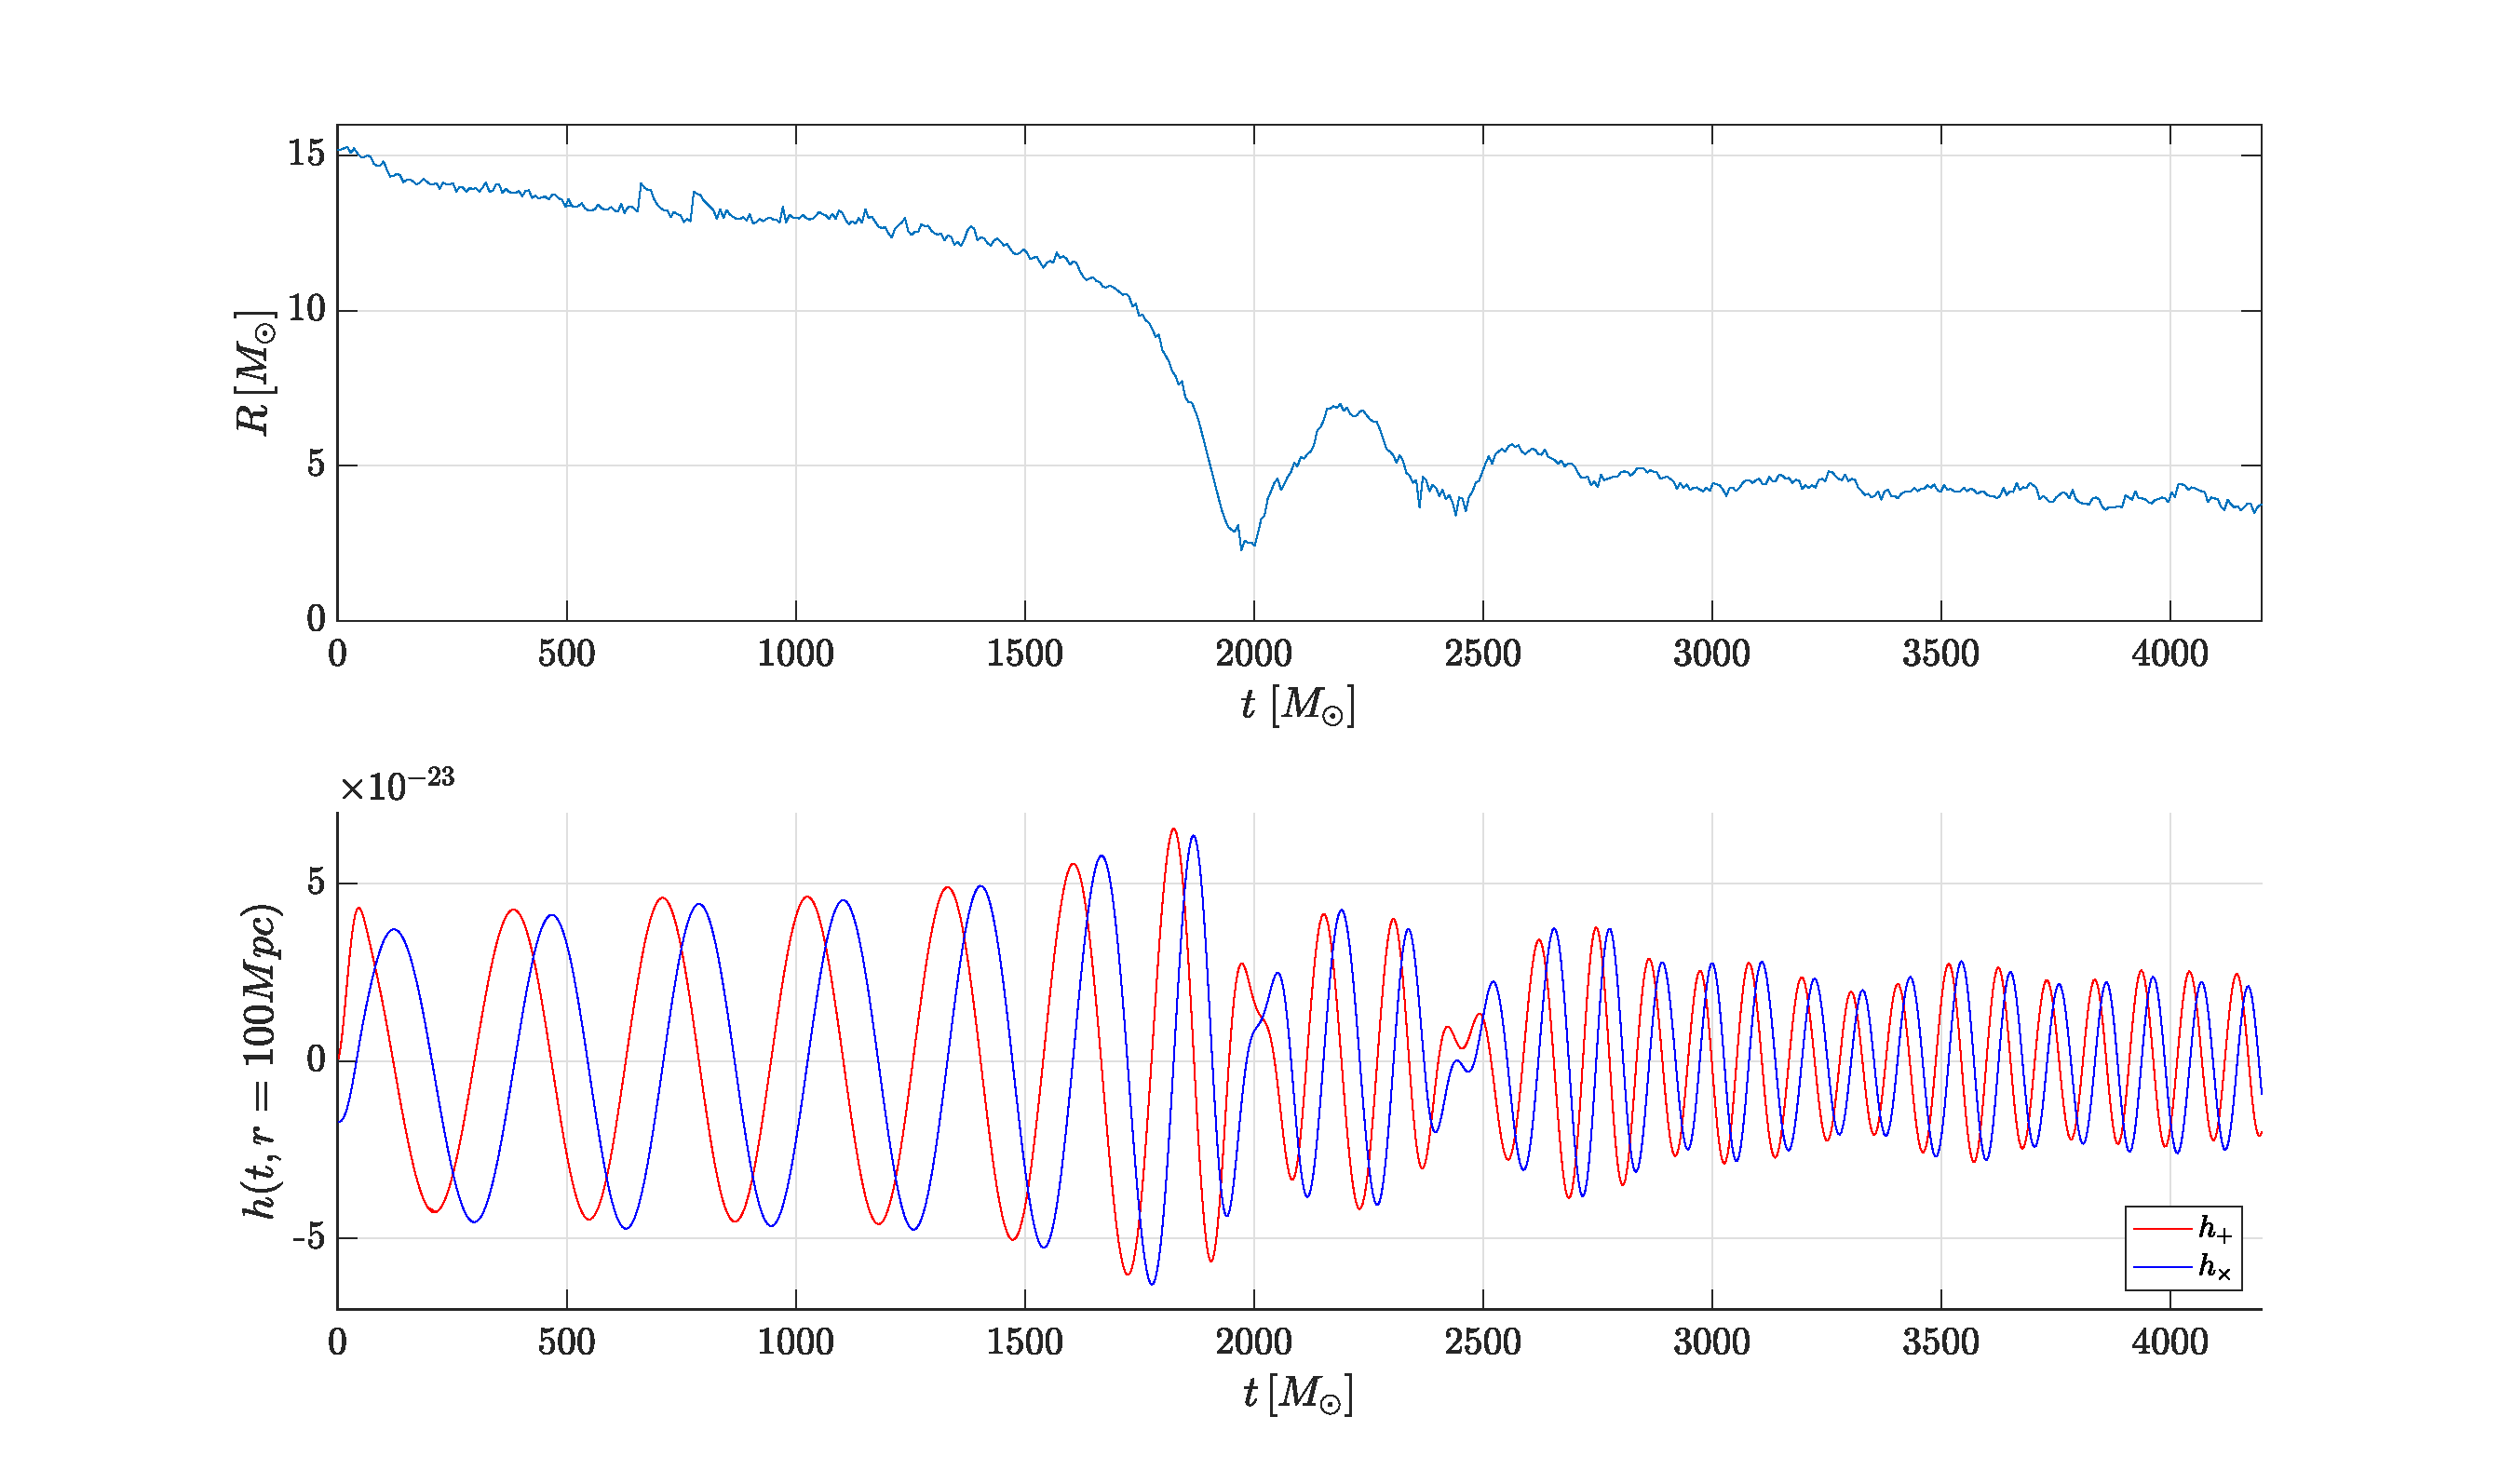
\includegraphics[scale=0.3,width=1\textwidth]{bns.eps}
    \end{figure}
    \end{widepage}
\end{frame}

\begin{frame}{Rest Mass Density Evolution}
%/Users/lorenzosperi/Documents/GitHub/thesis/gw/animate
\begin{figure}
    \centering
    \animategraphics[loop,autoplay,scale=0.35]{8}{/Users/lorenzosperi/Documents/GitHub/thesis/binary_ns_video/rho_000000}{001}{391}
    \end{figure}
\end{frame}

\section{Conclusions}
\begin{frame}{Conclusions}
\emph{\textbf{"Gravitational
waves will show us details of the bulk motion of
dense concentrations of energy"}}\\
\vspace{0.2cm} Kip S. Thorne
\begin{figure}
    \centering
    \animategraphics[loop,autoplay,scale=0.35]{24}{/Users/lorenzosperi/Documents/GitHub/thesis/gw/3d/frame-}{1}{62}
    \end{figure}
\end{frame}


\end{document}